% Options for packages loaded elsewhere
\PassOptionsToPackage{unicode}{hyperref}
\PassOptionsToPackage{hyphens}{url}
%
\documentclass[
]{article}
\usepackage{amsmath,amssymb}
\usepackage{iftex}
\ifPDFTeX
  \usepackage[T1]{fontenc}
  \usepackage[utf8]{inputenc}
  \usepackage{textcomp} % provide euro and other symbols
\else % if luatex or xetex
  \usepackage{unicode-math} % this also loads fontspec
  \defaultfontfeatures{Scale=MatchLowercase}
  \defaultfontfeatures[\rmfamily]{Ligatures=TeX,Scale=1}
\fi
\usepackage{lmodern}
\ifPDFTeX\else
  % xetex/luatex font selection
    \setmainfont[]{Arial}
\fi
% Use upquote if available, for straight quotes in verbatim environments
\IfFileExists{upquote.sty}{\usepackage{upquote}}{}
\IfFileExists{microtype.sty}{% use microtype if available
  \usepackage[]{microtype}
  \UseMicrotypeSet[protrusion]{basicmath} % disable protrusion for tt fonts
}{}
\makeatletter
\@ifundefined{KOMAClassName}{% if non-KOMA class
  \IfFileExists{parskip.sty}{%
    \usepackage{parskip}
  }{% else
    \setlength{\parindent}{0pt}
    \setlength{\parskip}{6pt plus 2pt minus 1pt}}
}{% if KOMA class
  \KOMAoptions{parskip=half}}
\makeatother
\usepackage{xcolor}
\usepackage[landscape,top=5cm,left=2.5cm,bottom=2cm,right=2.5cm,margin=1in]{geometry}
\usepackage{graphicx}
\makeatletter
\newsavebox\pandoc@box
\newcommand*\pandocbounded[1]{% scales image to fit in text height/width
  \sbox\pandoc@box{#1}%
  \Gscale@div\@tempa{\textheight}{\dimexpr\ht\pandoc@box+\dp\pandoc@box\relax}%
  \Gscale@div\@tempb{\linewidth}{\wd\pandoc@box}%
  \ifdim\@tempb\p@<\@tempa\p@\let\@tempa\@tempb\fi% select the smaller of both
  \ifdim\@tempa\p@<\p@\scalebox{\@tempa}{\usebox\pandoc@box}%
  \else\usebox{\pandoc@box}%
  \fi%
}
% Set default figure placement to htbp
\def\fps@figure{htbp}
\makeatother
\setlength{\emergencystretch}{3em} % prevent overfull lines
\providecommand{\tightlist}{%
  \setlength{\itemsep}{0pt}\setlength{\parskip}{0pt}}
\setcounter{secnumdepth}{-\maxdimen} % remove section numbering
\usepackage{graphicx}
\usepackage{xcolor}
\usepackage{eso-pic}
\usepackage{lipsum}
\definecolor{azuloscuro}{RGB}{0,51,102}
\definecolor{turquesa}{RGB}{0,174,239}
\usepackage{fancyhdr}
\pagestyle{fancy}
\fancyhf{}
\renewcommand{\headrulewidth}{0pt}
\fancyfoot[R]{\thepage}
\usepackage{booktabs}
\usepackage{longtable}
\usepackage{array}
\usepackage{multirow}
\usepackage{wrapfig}
\usepackage{float}
\usepackage{colortbl}
\usepackage{pdflscape}
\usepackage{tabu}
\usepackage{threeparttable}
\usepackage{threeparttablex}
\usepackage[normalem]{ulem}
\usepackage{makecell}
\usepackage{xcolor}
\usepackage{bookmark}
\IfFileExists{xurl.sty}{\usepackage{xurl}}{} % add URL line breaks if available
\urlstyle{same}
\hypersetup{
  hidelinks,
  pdfcreator={LaTeX via pandoc}}

\author{}
\date{\vspace{-2.5em}2025-05-23}

\begin{document}

\thispagestyle{empty}

\AddToShipoutPictureBG*{%
    \AtStockLowerLeft{%
        
\includegraphics[width=\paperwidth,height=\paperheight]{image.png}%
    }%
}

\AddToShipoutPicture*{%
    \AtStockUpperLeft{%
        \hspace*{4 cm}%
        \raisebox{-3.5cm}{
\includegraphics[height=0.6cm]{Logo_Portada.png}
}%
    }%
}

\vspace*{4cm}
\begin{flushleft}
    \hspace*{1.5cm}{\fontsize{38}{45}\selectfont\color{white}\textbf{Reporte Modelo de Inundación}}\\[0.8cm]
    \hspace*{1.5cm}{\fontsize{24}{30}\selectfont\color{white}Análisis de Portafolio}\\[1.2cm]
    \hspace*{1.5cm}{\fontsize{24}{30}\selectfont\color{white}Mash}\\[0.4cm]
    \hspace*{1.5cm}{\Large\color{white}Mayo 2025}
\end{flushleft}

\vfill
\begin{flushleft}
    \hspace*{1.5cm}{\small\color{white}Un negocio de Marsh McLennan}
\end{flushleft}

\clearpage

\noindent \textbf{\textcolor{turquesa}{\fontsize{16}{20}\selectfont Contenido}}

\noindent

\begin{enumerate}
    \item {\fontsize{11}{13}\selectfont Resumen \dotfill \pageref{sec:summary}}
    \item {\fontsize{11}{13}\selectfont Resultados \dotfill \pageref{sec:results}}
\end{enumerate}

\newpage

\noindent \textbf{\textcolor{turquesa}{\fontsize{16}{20}\selectfont Consideraciones}}
\vspace{0.5cm}

\noindent \fontsize{11}{13}\selectfont La tecnología utilizada y las
referencias proporcionadas para la generación de esta información se
basan en datos científicos, modelos matemáticos y experiencia codificada
de investigadores y especialistas en el área de Data Management.

\begin{itemize}
    \item {\fontsize{11}{13}\selectfont El presente informe, así como los análisis, modelos y predicciones que contiene este documento, ("Información"), se basan en datos provistos por MARSH a través de nuestro cliente: Mash y gestionados a través de la tecnología informática de evaluación de riesgos propiedad de JBA Risk Management.}
    \item {\fontsize{11}{13}\selectfont Es importante mencionar que la exactitud de las predicciones depende en gran medida de la precisión y calidad de los datos proporcionados por el cliente: Mash a los especialistas de MARSH.}
    \item {\fontsize{11}{13}\selectfont La gestión de la información proporcionada por Mash se realiza a través del licenciamiento de MARSH en JBA Risk Management, haciendo uso de los marcos regulatorios para la protección de información confidencial; prohibiendo su distribución con terceros sin el previo consentimiento escrito de MARSH y JBA Risk Management.}
    \item {\fontsize{11}{13}\selectfont La Información descrita dentro del reporte generado por Marsh, sólo puede ser utilizada con el propósito de estudio e interpretación de resultados para: Mash Este documento no puede ser utilizada bajo ninguna circunstancia en el desarrollo y/ o calibración de cualquier oferta de productos o servicios que compita con JBA Risk Management y MARSH.}
\end{itemize}

\fontsize{11}{13}\selectfont Los mapas globales de inundaciones de JBA
Risk Management, y la gestión de información de Marsh, proporcionan
información indicativa sobre la extensión y profundidad de las
inundaciones para ríos no defendidos y riesgos de inundaciones de aguas
superficiales para los periodos de retorno de 20, 50, 100, 200, 500 y
1.500 años. Los datos digitales de elevación subyacentes son una
combinación de Modelos Digitales del Terreno (MDT) de una variedad de
fuentes.

\fontsize{11}{13}\selectfont Para las actualizaciones cartográficas
posteriores a 2023, se utiliza ampliamente el DTMlite de Airbus
WorldDEM. La cartografía de los riesgos de inundación se proporciona a
escala mundial con una resolución de 30 m para todos los ríos y para las
aguas superficiales. Los mapas se crean simulando los totales de
precipitaciones de diseño y los volúmenes de caudal de los ríos,
permitiendo que la inundación asociada a cada uno de ellos se extienda
por el terreno circundante mediante un software de modelización
hidráulica. Con el fin de estimar los caudales de los ríos y las
cantidades de lluvia para cada período de retorno en cualquier lugar del
mundo, JBA ha desarrollado modelos hidrológicos adecuados para la
cartografía a escala mundial.

\newpage

\noindent \textbf{\textcolor{azuloscuro}{\fontsize{28}{32}\selectfont Resumen}}
\label{sec:summary} \vspace{0.5cm}

\fontsize{11}{13}\selectfont Este informe probabilístico sirve como
herramienta para evaluar y cuantificar su riesgo a inundación. Este
análisis utiliza modelos matemáticos y estadísticos para simular
diferentes escenarios de inundación y determinar la probabilidad de que
ocurran en un momento dado. Para la creación de este reporte se utilizan
datos históricos, topográficos y de precipitación sobre zonas
determinadas. Los resultados se presentan para los periodos de retorno
de 20, 50, 100, 200, 500 y 1500 años con resultados que muestran las
áreas afectadas y la dimensión de esta.

\fontsize{11}{13}\selectfont El propósito de este informe es
proporcionar a Mash una Evaluación de Riesgo de Inundación.

\fontsize{11}{13}\selectfont El alcance del proyecto incluye importar
directamente los datos de entrada, según lo proporcionado por el
cliente, en el modelo y ejecutar los análisis. El conjunto de eventos de
inundación global de JBA permite examinar los patrones de inundación y
evaluar las exposiciones a escala regional, continental y global para
Mash. El modelo utiliza métodos estadísticos sofisticados, junto con
procesos de modelos físicos de lluvia y escorrentía, para capturar las
posibles correlaciones espaciales y temporales de inundaciones causadas
por ciclones tropicales, precipitaciones extremas y caudal de río. Las
zonas de acumulación hidrológica se utilizan para comprender mejor las
correlaciones de inundación e identificar áreas que pueden verse
afectadas simultáneamente por el mismo evento, además proporcionan una
unidad geográfica alternativa a los límites de la administración
política para el análisis de agregación y acumulación. Los resultados
por inundación de río representan inundaciones causadas por toda agua
que este en movimiento (ríos, caños, drenajes). Los resultados por agua
superficial representan inundaciones causadas por estancamiento de agua
y desbordamiento de masas de agua que se hallan depositadas en
depresiones de un terreno.

\fontsize{11}{13}\selectfont Los modelos catastróficos a nivel país de
JBA incorporan sus datos de inundaciones de alta resolución y
proyecciones climáticas reconocidas internacionalmente, lo que permite
evaluar la línea de base actual y el riesgo futuro de inundación de ríos
y aguas superficiales con confianza para todos los países del mundo.

\fontsize{11}{13}\selectfont Los resultados proporcionados por este
informe son importantes para tomar decisiones sobre la prevención del
uso del suelo, la construcción de infraestructura y la planificación de
recuperación después de inundación. Se recomienda tomar medidas
preventivas y de mitigación para reducir el impacto de las inundaciones
y proteger vida humana, propiedad e infraestructura, así como tomarlo en
cuenta para salvaguardar maquinaria, insumos o inventarios importantes
que puedan causar la interrupción total o parcial del negocio.

\newpage

\noindent \textbf{\textcolor{azuloscuro}{\fontsize{11}{13}\selectfont Para Mash se tuvieron en cuenta las siguientes consideraciones:}}
\vspace{0.5cm}

\begin{table}[!h]
\centering\begingroup\fontsize{11}{13}\selectfont

\resizebox{\ifdim\width>\linewidth\linewidth\else\width\fi}{!}{
\begin{tabular}{cccccc}
\toprule
\cellcolor{azuloscuro}{\textcolor{white}{ID}} & \cellcolor{azuloscuro}{\textcolor{white}{Name}} & \cellcolor{azuloscuro}{\textcolor{white}{Country}} & \cellcolor{azuloscuro}{\textcolor{white}{Latitude}} & \cellcolor{azuloscuro}{\textcolor{white}{Longitude}} & \cellcolor{azuloscuro}{\textcolor{white}{Buffer}}\\
\midrule
\cellcolor{gray!10}{1} & \cellcolor{gray!10}{Centro ABC} & \cellcolor{gray!10}{Dominican Republic} & \cellcolor{gray!10}{18.52248} & \cellcolor{gray!10}{-69.74553} & \cellcolor{gray!10}{Polygon}\\
2 & Centro xyz & Dominican Republic & 18.52779 & -69.83790 & Polygon\\
\bottomrule
\end{tabular}}
\endgroup{}
\end{table}

\vspace{1cm}

\begin{table}[!h]
\centering
\begin{tabular}{lll}
\toprule
\multicolumn{1}{>{\centering\arraybackslash}m{0.3\textwidth}}{\cellcolor{azuloscuro}{\color{white}\textbf{Centro 2SDF}}} & \multicolumn{1}{>{\centering\arraybackslash}m{0.3\textwidth}}{\cellcolor{azuloscuro}{\color{white}\textbf{Centro 2SDF3}}} & \multicolumn{1}{>{\centering\arraybackslash}m{0.3\textwidth}}{\cellcolor{azuloscuro}{\color{white}\textbf{Centro 3ABC}}}\\
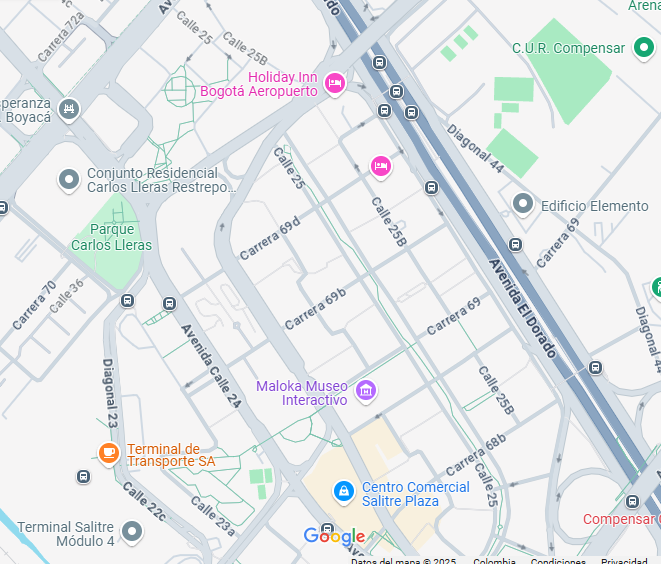
\includegraphics[width=0.3\textwidth]{temp_maps/Centro 2SDF.png} & 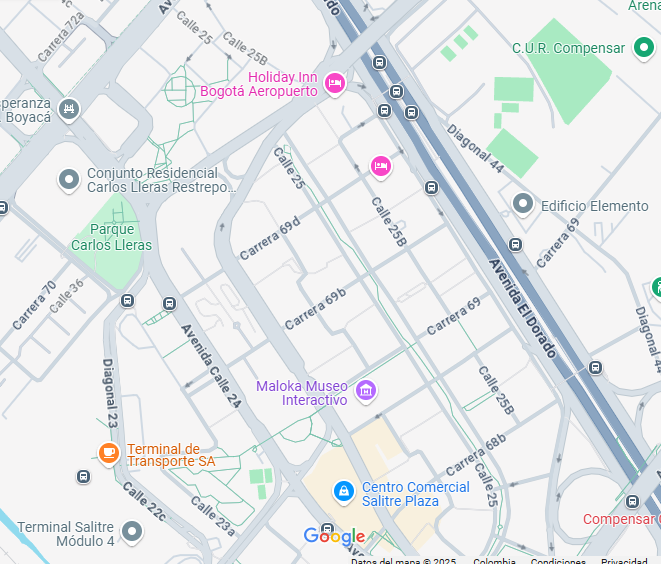
\includegraphics[width=0.3\textwidth]{temp_maps/Centro 2SDF3.png} & 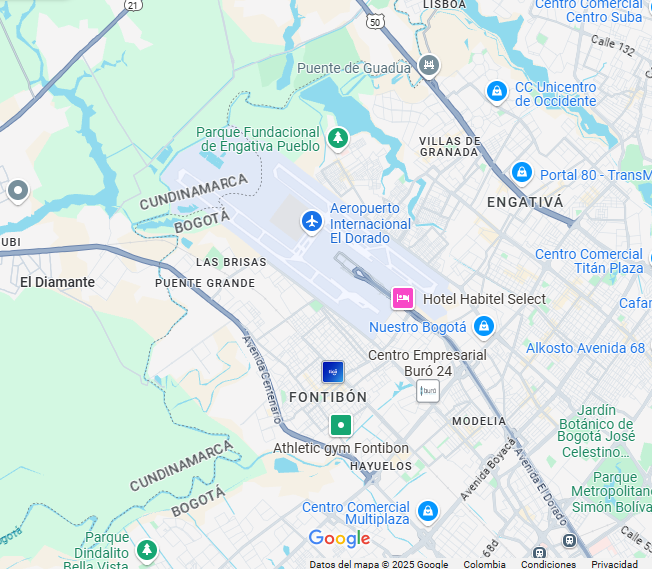
\includegraphics[width=0.3\textwidth]{temp_maps/Centro 3ABC.png}\\
\bottomrule
\end{tabular}
\end{table}
\vspace{0.8cm}
\newpage
\vspace*{\fill}
\begin{table}[!h]
\centering
\begin{tabular}{lll}
\toprule
\multicolumn{1}{>{\centering\arraybackslash}m{0.3\textwidth}}{\cellcolor{azuloscuro}{\color{white}\textbf{Centro ABC}}} & \multicolumn{1}{>{\centering\arraybackslash}m{0.3\textwidth}}{\cellcolor{azuloscuro}{\color{white}\textbf{Centro ABC3}}} & \multicolumn{1}{>{\centering\arraybackslash}m{0.3\textwidth}}{\cellcolor{azuloscuro}{\color{white}\textbf{Centro ABC3d}}}\\
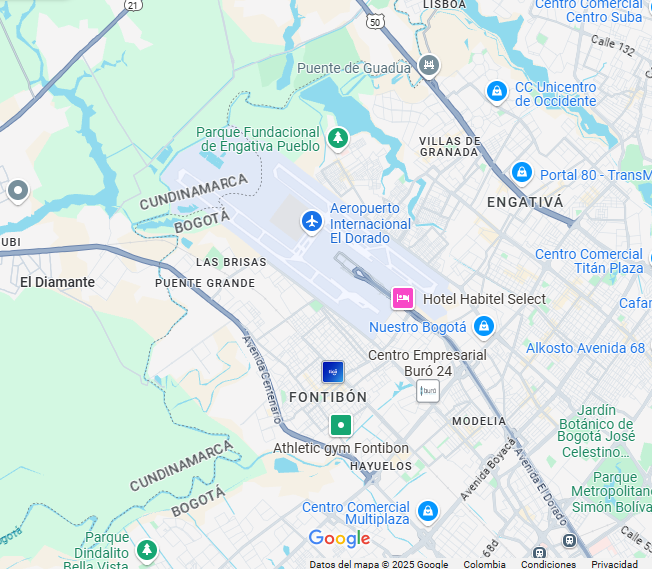
\includegraphics[width=0.3\textwidth]{temp_maps/Centro ABC.png} & 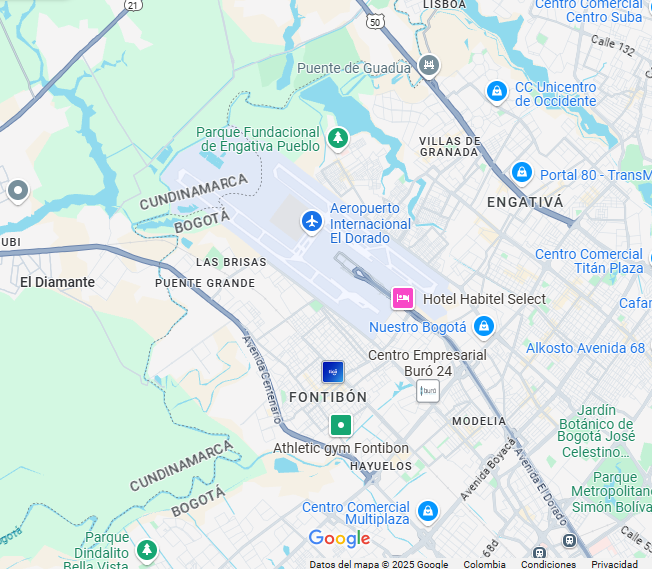
\includegraphics[width=0.3\textwidth]{temp_maps/Centro ABC3.png} & 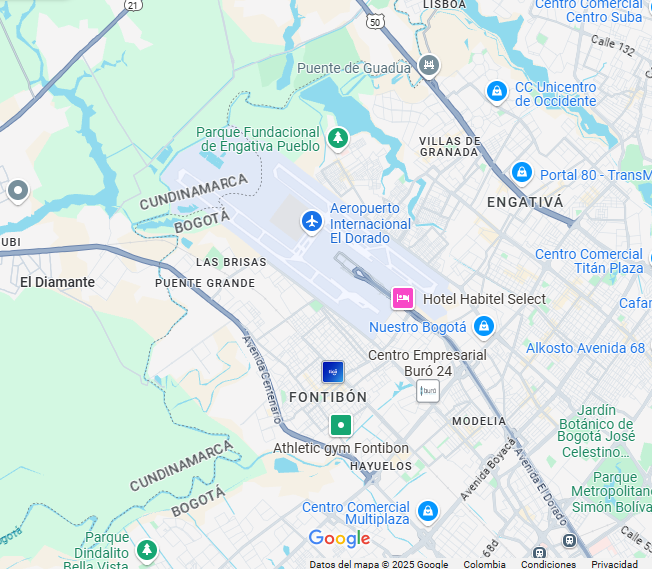
\includegraphics[width=0.3\textwidth]{temp_maps/Centro ABC3d.png}\\
\bottomrule
\end{tabular}
\end{table}
\vspace*{\fill}
\newpage
\vspace*{\fill}
\begin{table}[!h]
\centering
\begin{tabular}{lll}
\toprule
\multicolumn{1}{>{\centering\arraybackslash}m{0.3\textwidth}}{\cellcolor{azuloscuro}{\color{white}\textbf{Centro dABC}}} & \multicolumn{1}{>{\centering\arraybackslash}m{0.3\textwidth}}{\cellcolor{azuloscuro}{\color{white}\textbf{Centro fgvSD}}} & \multicolumn{1}{>{\centering\arraybackslash}m{0.3\textwidth}}{\cellcolor{azuloscuro}{\color{white}\textbf{Centro fSD3}}}\\
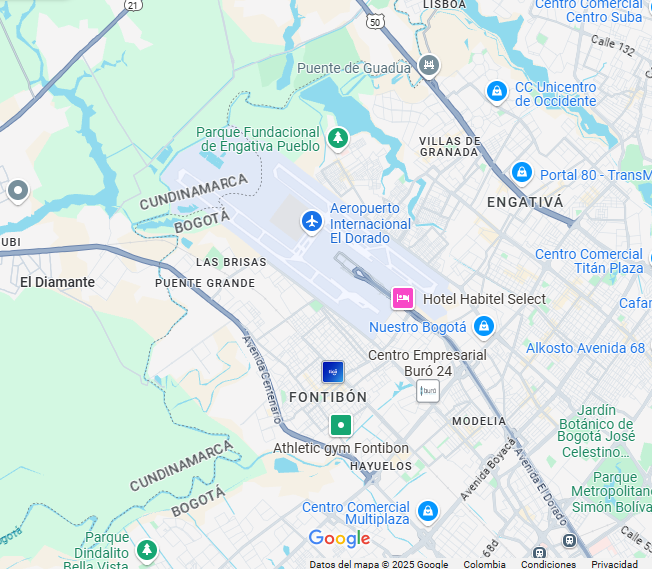
\includegraphics[width=0.3\textwidth]{temp_maps/Centro dABC.png} & 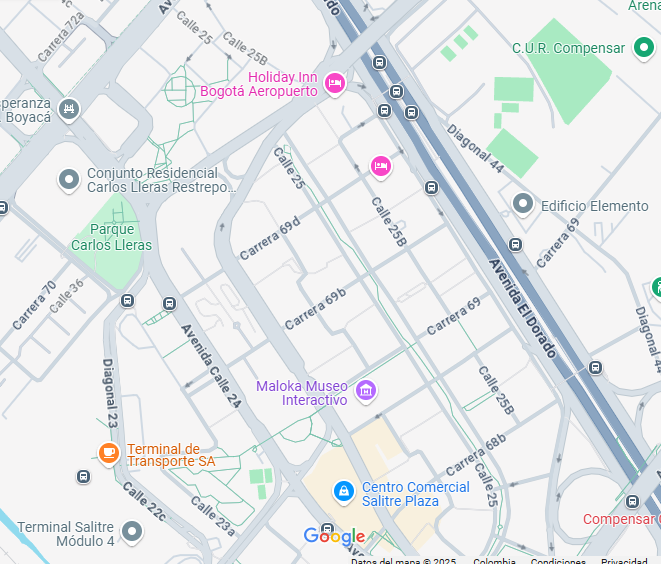
\includegraphics[width=0.3\textwidth]{temp_maps/Centro fgvSD.png} & 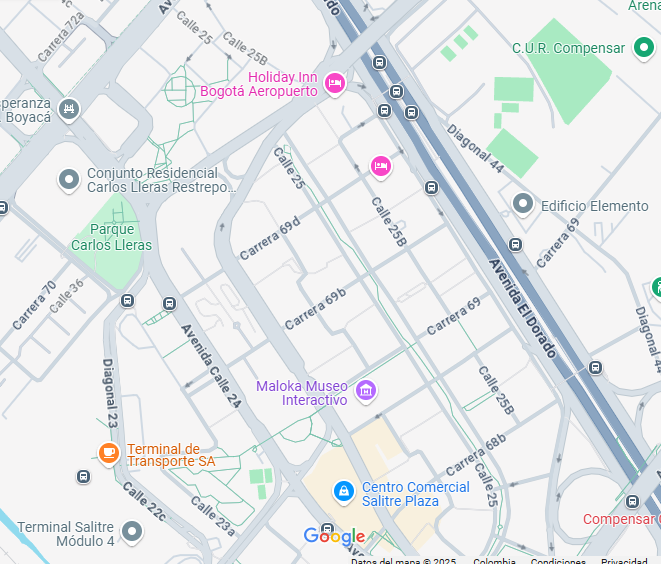
\includegraphics[width=0.3\textwidth]{temp_maps/Centro fSD3.png}\\
\bottomrule
\end{tabular}
\end{table}
\vspace*{\fill}
\newpage
\vspace*{\fill}
\begin{table}[!h]
\centering
\begin{tabular}{lll}
\toprule
\multicolumn{1}{>{\centering\arraybackslash}m{0.3\textwidth}}{\cellcolor{azuloscuro}{\color{white}\textbf{Centro rABC3}}} & \multicolumn{1}{>{\centering\arraybackslash}m{0.3\textwidth}}{\cellcolor{azuloscuro}{\color{white}\textbf{Centro SDF}}} & \multicolumn{1}{>{\centering\arraybackslash}m{0.3\textwidth}}{\cellcolor{azuloscuro}{\color{white}\textbf{Centro SDF3}}}\\
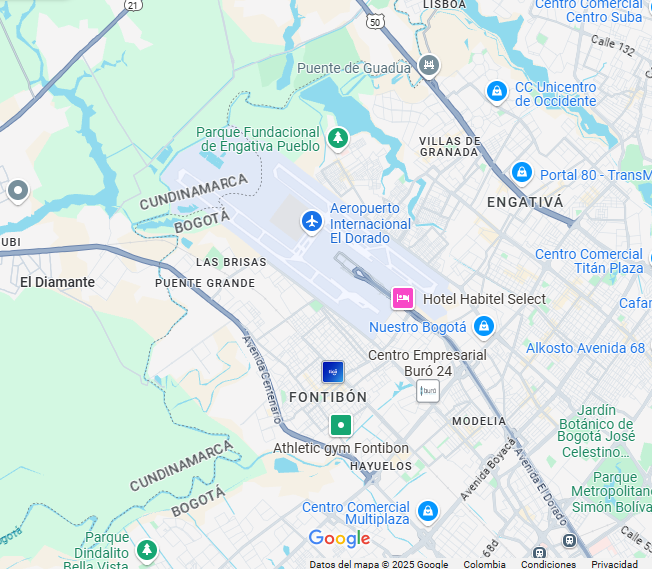
\includegraphics[width=0.3\textwidth]{temp_maps/Centro rABC3.png} & 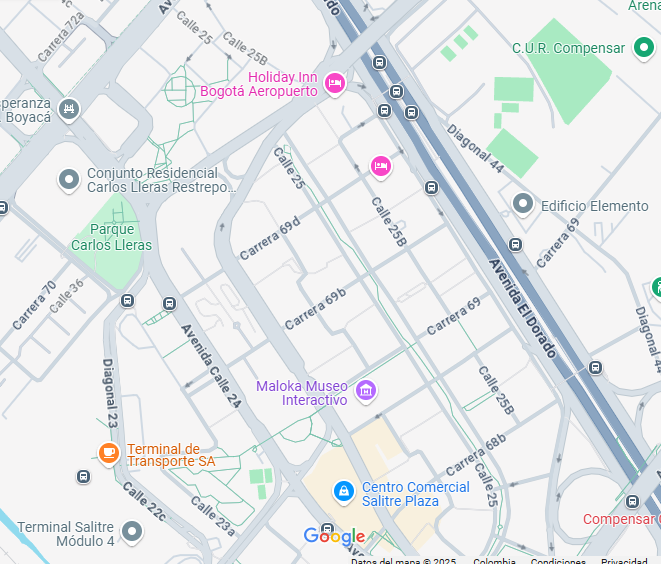
\includegraphics[width=0.3\textwidth]{temp_maps/Centro SDF.png} & 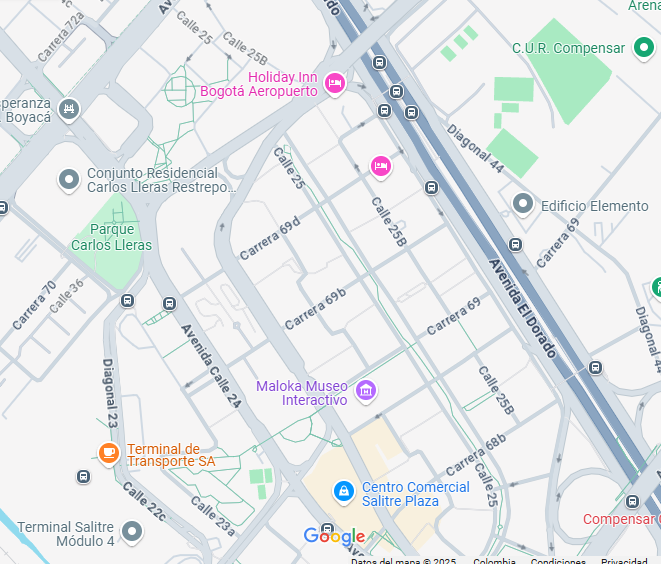
\includegraphics[width=0.3\textwidth]{temp_maps/Centro SDF3.png}\\
\bottomrule
\end{tabular}
\end{table}
\vspace*{\fill}
\newpage
\vspace*{\fill}
\begin{table}[!h]
\centering
\begin{tabular}{lll}
\toprule
\multicolumn{1}{>{\centering\arraybackslash}m{0.3\textwidth}}{\cellcolor{azuloscuro}{\color{white}\textbf{Centro SDfF}}} & \multicolumn{1}{>{\centering\arraybackslash}m{0.3\textwidth}}{\cellcolor{azuloscuro}{\color{white}\textbf{Centro vABC3}}} & \multicolumn{1}{>{\centering\arraybackslash}m{0.3\textwidth}}{\cellcolor{azuloscuro}{\color{white}\textbf{Centro vrABC}}}\\
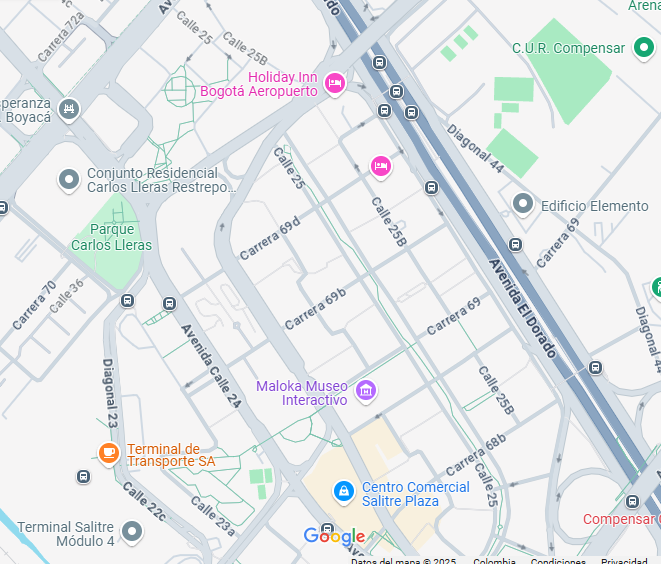
\includegraphics[width=0.3\textwidth]{temp_maps/Centro SDfF.png} & 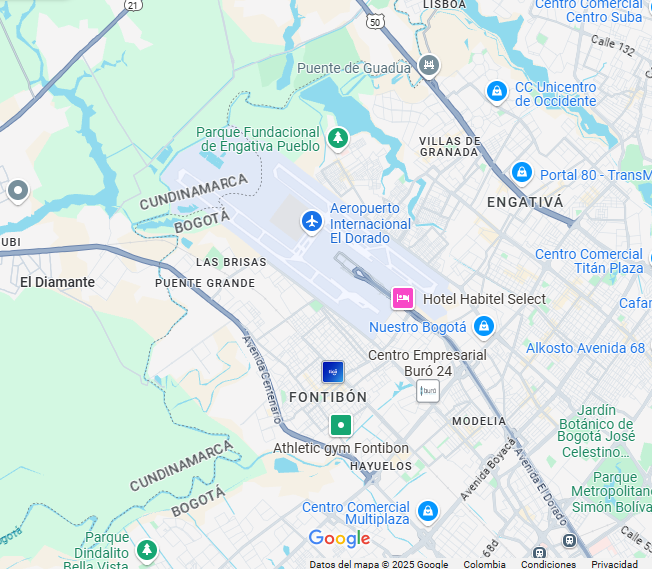
\includegraphics[width=0.3\textwidth]{temp_maps/Centro vABC3.png} & 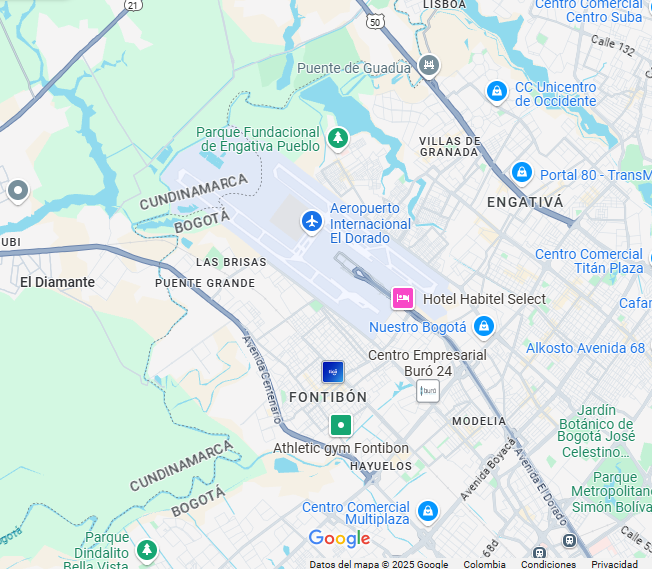
\includegraphics[width=0.3\textwidth]{temp_maps/Centro vrABC.png}\\
\bottomrule
\end{tabular}
\end{table}
\vspace*{\fill}
\newpage
\vspace*{\fill}
\begin{table}[!h]
\centering
\begin{tabular}{lll}
\toprule
\multicolumn{1}{>{\centering\arraybackslash}m{0.3\textwidth}}{\cellcolor{azuloscuro}{\color{white}\textbf{Centro vSDF3}}} & \multicolumn{1}{>{\centering\arraybackslash}m{0.3\textwidth}}{\cellcolor{azuloscuro}{\color{white}\textbf{Centro XYZ}}} & \\
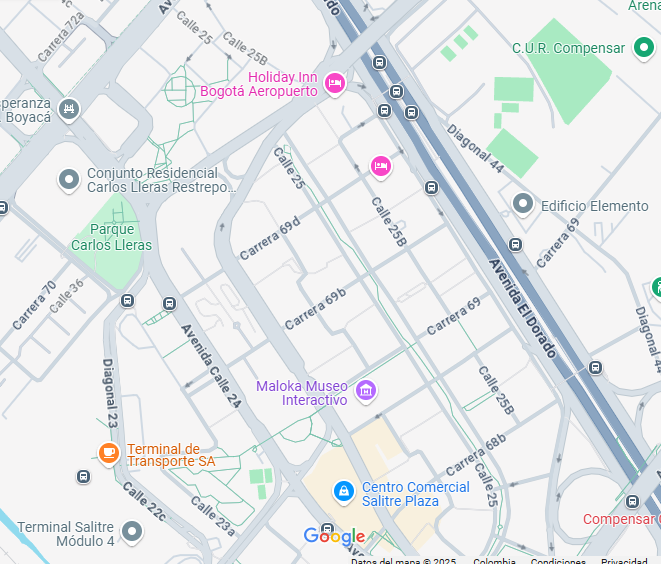
\includegraphics[width=0.3\textwidth]{temp_maps/Centro vSDF3.png} & 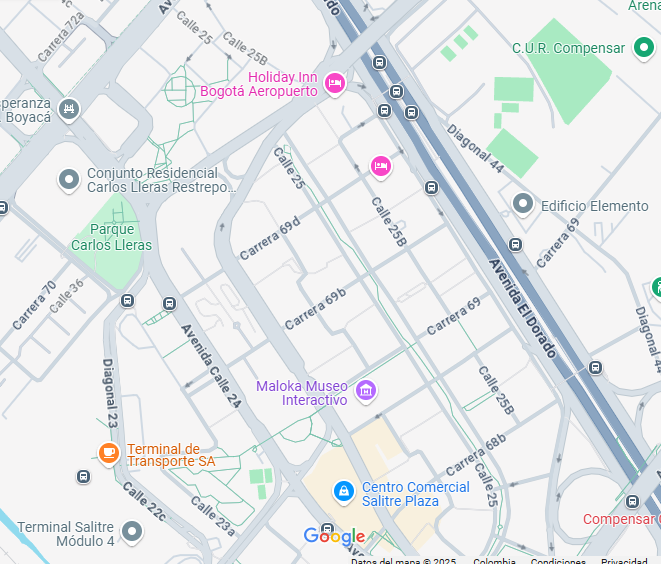
\includegraphics[width=0.3\textwidth]{temp_maps/Centro XYZ.png} & \\
\bottomrule
\end{tabular}
\end{table}
\vspace*{\fill}

\newpage

\noindent \textbf{\textcolor{azuloscuro}{\fontsize{28}{32}\selectfont Resultados}}
\label{sec:results}

\vspace{0.3cm}

\textbf{\textcolor{turquesa}{\fontsize{16}{20}\selectfont Centro ABC}}

\fontsize{11}{13}\selectfont La siguiente tabla muestra la inundación
promedio y máxima en metros para la ubicación Centro ABC.

\begin{table}[!h]
\centering\begingroup\fontsize{11}{13}\selectfont

\resizebox{\ifdim\width>\linewidth\linewidth\else\width\fi}{!}{
\begin{tabular}{cccccccc}
\toprule
\multicolumn{2}{c}{\cellcolor{azuloscuro}{\textcolor{white}{Periodo de Retorno}}} & \multicolumn{3}{c}{\cellcolor{azuloscuro}{\textcolor{white}{Profundidad Inundación Ríos}}} & \multicolumn{3}{c}{\cellcolor{azuloscuro}{\textcolor{white}{Profundidad de Aguas Superficiales}}} \\
\cmidrule(l{3pt}r{3pt}){1-2} \cmidrule(l{3pt}r{3pt}){3-5} \cmidrule(l{3pt}r{3pt}){6-8}
\cellcolor{azuloscuro}{\textcolor{white}{Año}} & \cellcolor{azuloscuro}{\textcolor{white}{Probabilidad}} & \cellcolor{azuloscuro}{\textcolor{white}{Área Afectada (\%)}} & \cellcolor{azuloscuro}{\textcolor{white}{Promedio (m)}} & \cellcolor{azuloscuro}{\textcolor{white}{Máxima (m)}} & \cellcolor{azuloscuro}{\textcolor{white}{Área Afectada  (\%)}} & \cellcolor{azuloscuro}{\textcolor{white}{Promedio  (m)}} & \cellcolor{azuloscuro}{\textcolor{white}{Máxima  (m)}}\\
\midrule
\cellcolor{gray!10}{20} & \cellcolor{gray!10}{1\%} & \cellcolor{gray!10}{20} & \cellcolor{gray!10}{20} & \cellcolor{gray!10}{20} & \cellcolor{gray!10}{20} & \cellcolor{gray!10}{20} & \cellcolor{gray!10}{20}\\
50 & 10\% & 50 & 50 & 50 & 50 & 50 & 50\\
\cellcolor{gray!10}{100} & \cellcolor{gray!10}{1\%} & \cellcolor{gray!10}{100} & \cellcolor{gray!10}{100} & \cellcolor{gray!10}{100} & \cellcolor{gray!10}{100} & \cellcolor{gray!10}{100} & \cellcolor{gray!10}{100}\\
200 & 10\% & 200 & 200 & 200 & 200 & 200 & 200\\
\cellcolor{gray!10}{500} & \cellcolor{gray!10}{1\%} & \cellcolor{gray!10}{500} & \cellcolor{gray!10}{500} & \cellcolor{gray!10}{500} & \cellcolor{gray!10}{500} & \cellcolor{gray!10}{500} & \cellcolor{gray!10}{500}\\
\addlinespace
1500 & 10\% & 1500 & 1500 & 1500 & 1500 & 1500 & 1500\\
\bottomrule
\end{tabular}}
\endgroup{}
\end{table}

\begin{center}
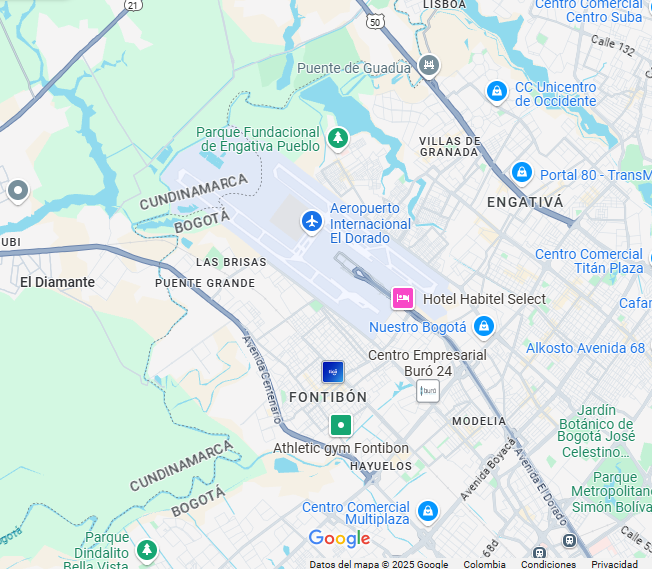
\includegraphics[width=0.37\textwidth]{temp_maps/Centro ABC.png}
\end{center}

\newpage

\textbf{\textcolor{turquesa}{\fontsize{16}{20}\selectfont Centro ABC – Períodos de     Retorno}}

\vspace{0.3cm}
\begin{center}
\begin{table}[!h]
\centering
\begin{tabular}{lll}
\toprule
\multicolumn{1}{>{\centering\arraybackslash}m{0.3\textwidth}}{\cellcolor{azuloscuro}{\color{white}\textbf{1-20}}} & \multicolumn{1}{>{\centering\arraybackslash}m{0.3\textwidth}}{\cellcolor{azuloscuro}{\color{white}\textbf{1-50}}} & \multicolumn{1}{>{\centering\arraybackslash}m{0.3\textwidth}}{\cellcolor{azuloscuro}{\color{white}\textbf{1-100}}}\\
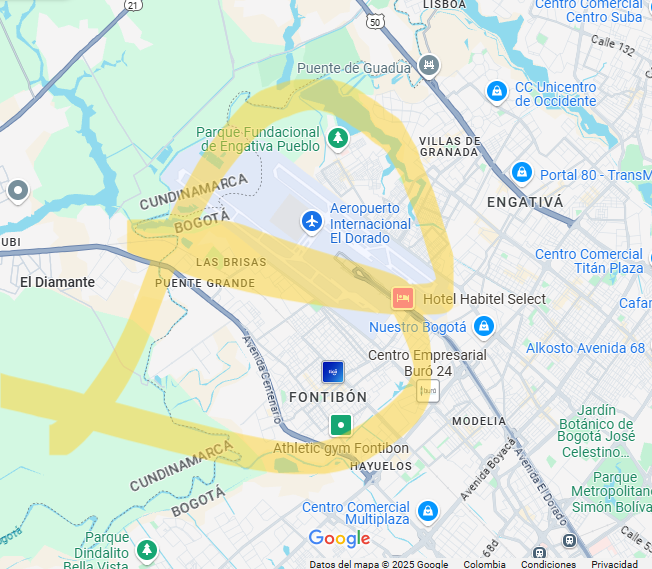
\includegraphics[width=0.3\textwidth]{C:/Users/windows/Documents/GitHub/Problem_Set_1/Flood Report/Flood/1. Mapas/Cliente ABC/Centro ABC/1-20.png} & 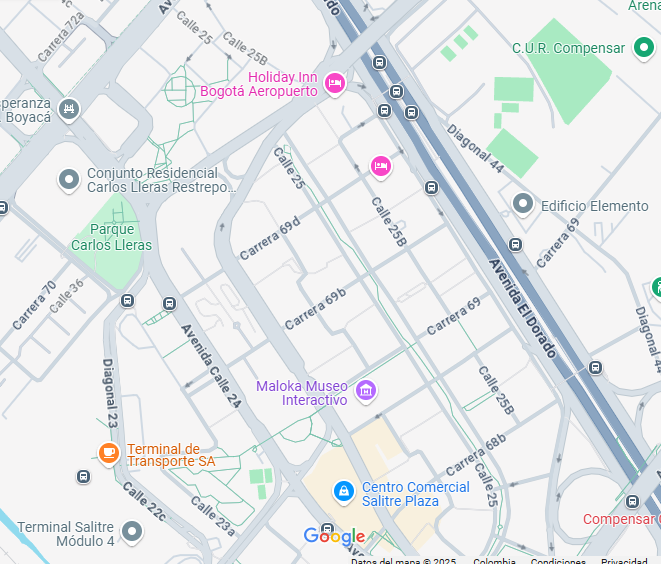
\includegraphics[width=0.3\textwidth]{C:/Users/windows/Documents/GitHub/Problem_Set_1/Flood Report/Flood/1. Mapas/Cliente ABC/Centro ABC/1-50.png} & \includegraphics[width=0.3\textwidth]{C:/Users/windows/Documents/GitHub/Problem_Set_1/Flood Report/Flood/1. Mapas/Cliente ABC/Centro ABC/1-100.png}\\
\bottomrule
\end{tabular}
\end{table} 

\begin{table}[!h]
\centering
\begin{tabular}{lll}
\toprule
\multicolumn{1}{>{\centering\arraybackslash}m{0.3\textwidth}}{\cellcolor{azuloscuro}{\color{white}\textbf{1-200}}} & \multicolumn{1}{>{\centering\arraybackslash}m{0.3\textwidth}}{\cellcolor{azuloscuro}{\color{white}\textbf{1-500}}} & \\
\includegraphics[width=0.3\textwidth]{C:/Users/windows/Documents/GitHub/Problem_Set_1/Flood Report/Flood/1. Mapas/Cliente ABC/Centro ABC/1-200.png} & \includegraphics[width=0.3\textwidth]{C:/Users/windows/Documents/GitHub/Problem_Set_1/Flood Report/Flood/1. Mapas/Cliente ABC/Centro ABC/1-500.png} & \\
\bottomrule
\end{tabular}
\end{table} 

\end{center}
\vspace{0.5cm}
\newpage

\textbf{\textcolor{turquesa}{\fontsize{16}{20}\selectfont Centro SDF}}

\fontsize{11}{13}\selectfont La siguiente tabla muestra la inundación
promedio y máxima en metros para la ubicación Centro SDF.

\begin{table}[!h]
\centering\begingroup\fontsize{11}{13}\selectfont

\resizebox{\ifdim\width>\linewidth\linewidth\else\width\fi}{!}{
\begin{tabular}{cccccccc}
\toprule
\multicolumn{2}{c}{\cellcolor{azuloscuro}{\textcolor{white}{Periodo de Retorno}}} & \multicolumn{3}{c}{\cellcolor{azuloscuro}{\textcolor{white}{Profundidad Inundación Ríos}}} & \multicolumn{3}{c}{\cellcolor{azuloscuro}{\textcolor{white}{Profundidad de Aguas Superficiales}}} \\
\cmidrule(l{3pt}r{3pt}){1-2} \cmidrule(l{3pt}r{3pt}){3-5} \cmidrule(l{3pt}r{3pt}){6-8}
\cellcolor{azuloscuro}{\textcolor{white}{Año}} & \cellcolor{azuloscuro}{\textcolor{white}{Probabilidad}} & \cellcolor{azuloscuro}{\textcolor{white}{Área Afectada (\%)}} & \cellcolor{azuloscuro}{\textcolor{white}{Promedio (m)}} & \cellcolor{azuloscuro}{\textcolor{white}{Perdida (m)}} & \cellcolor{azuloscuro}{\textcolor{white}{Área Afectada  (\%)}} & \cellcolor{azuloscuro}{\textcolor{white}{Promedio  (m)}} & \cellcolor{azuloscuro}{\textcolor{white}{Perdidaa (m)}}\\
\midrule
\cellcolor{gray!10}{20} & \cellcolor{gray!10}{1\%} & \cellcolor{gray!10}{20} & \cellcolor{gray!10}{340} & \cellcolor{gray!10}{4230} & \cellcolor{gray!10}{230} & \cellcolor{gray!10}{320} & \cellcolor{gray!10}{320}\\
50 & 10\% & 50 & 4530 & 4530 & 530 & 350 & 350\\
\cellcolor{gray!10}{100} & \cellcolor{gray!10}{1\%} & \cellcolor{gray!10}{100} & \cellcolor{gray!10}{4100} & \cellcolor{gray!10}{4130} & \cellcolor{gray!10}{1300} & \cellcolor{gray!10}{3100} & \cellcolor{gray!10}{3100}\\
200 & 10\% & 200 & 4300 & 4300 & 3200 & 3200 & 3200\\
\cellcolor{gray!10}{500} & \cellcolor{gray!10}{1\%} & \cellcolor{gray!10}{500} & \cellcolor{gray!10}{4300} & \cellcolor{gray!10}{4300} & \cellcolor{gray!10}{3500} & \cellcolor{gray!10}{3500} & \cellcolor{gray!10}{3500}\\
\addlinespace
1500 & 10\% & 1500 & 43500 & 13500 & 31500 & 31500 & 13500\\
\bottomrule
\end{tabular}}
\endgroup{}
\end{table}

\begin{center}
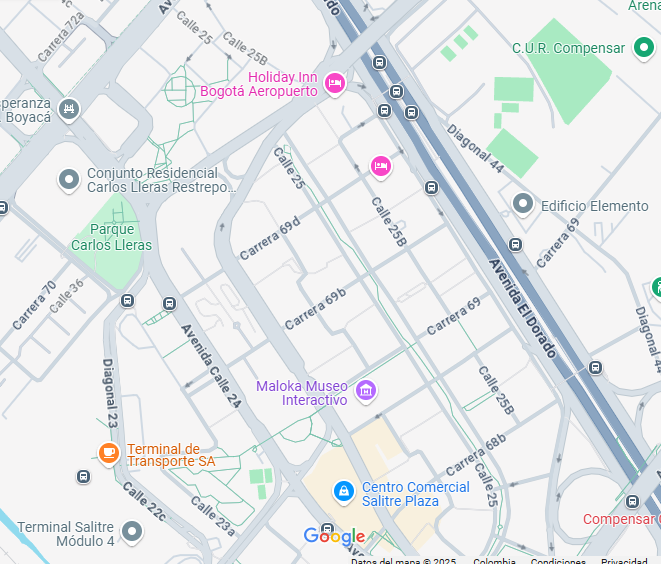
\includegraphics[width=0.37\textwidth]{temp_maps/Centro SDF.png}
\end{center}

\newpage

\textbf{\textcolor{turquesa}{\fontsize{16}{20}\selectfont Centro XYZ}}

\fontsize{11}{13}\selectfont La siguiente tabla muestra la inundación
promedio y máxima en metros para la ubicación Centro XYZ.

\begin{table}[!h]
\centering\begingroup\fontsize{11}{13}\selectfont

\resizebox{\ifdim\width>\linewidth\linewidth\else\width\fi}{!}{
\begin{tabular}{cccccccc}
\toprule
\multicolumn{2}{c}{\cellcolor{azuloscuro}{\textcolor{white}{Periodo de Retorno}}} & \multicolumn{3}{c}{\cellcolor{azuloscuro}{\textcolor{white}{Profundidad Inundación Ríos}}} & \multicolumn{3}{c}{\cellcolor{azuloscuro}{\textcolor{white}{Profundidad de Aguas Superficiales}}} \\
\cmidrule(l{3pt}r{3pt}){1-2} \cmidrule(l{3pt}r{3pt}){3-5} \cmidrule(l{3pt}r{3pt}){6-8}
\cellcolor{azuloscuro}{\textcolor{white}{Año}} & \cellcolor{azuloscuro}{\textcolor{white}{Probabilidad}} & \cellcolor{azuloscuro}{\textcolor{white}{Área Afectada (\%)}} & \cellcolor{azuloscuro}{\textcolor{white}{Promedio (m)}} & \cellcolor{azuloscuro}{\textcolor{white}{Máxima (m)}} & \cellcolor{azuloscuro}{\textcolor{white}{Área Afectada  (\%)}} & \cellcolor{azuloscuro}{\textcolor{white}{Promedio  (m)}} & \cellcolor{azuloscuro}{\textcolor{white}{Máxima  (m)}}\\
\midrule
\cellcolor{gray!10}{20} & \cellcolor{gray!10}{1\%} & \cellcolor{gray!10}{20} & \cellcolor{gray!10}{30} & \cellcolor{gray!10}{230} & \cellcolor{gray!10}{230} & \cellcolor{gray!10}{320} & \cellcolor{gray!10}{320}\\
50 & 10\% & 50 & 530 & 530 & 530 & 350 & 350\\
\cellcolor{gray!10}{100} & \cellcolor{gray!10}{1\%} & \cellcolor{gray!10}{100} & \cellcolor{gray!10}{1300} & \cellcolor{gray!10}{1300} & \cellcolor{gray!10}{1300} & \cellcolor{gray!10}{3100} & \cellcolor{gray!10}{3100}\\
200 & 10\% & 200 & 2300 & 2300 & 3200 & 3200 & 3200\\
\cellcolor{gray!10}{500} & \cellcolor{gray!10}{1\%} & \cellcolor{gray!10}{500} & \cellcolor{gray!10}{5300} & \cellcolor{gray!10}{5300} & \cellcolor{gray!10}{3500} & \cellcolor{gray!10}{3500} & \cellcolor{gray!10}{3500}\\
\addlinespace
1500 & 10\% & 1500 & 13500 & 13500 & 31500 & 31500 & 13500\\
\bottomrule
\end{tabular}}
\endgroup{}
\end{table}

\begin{center}
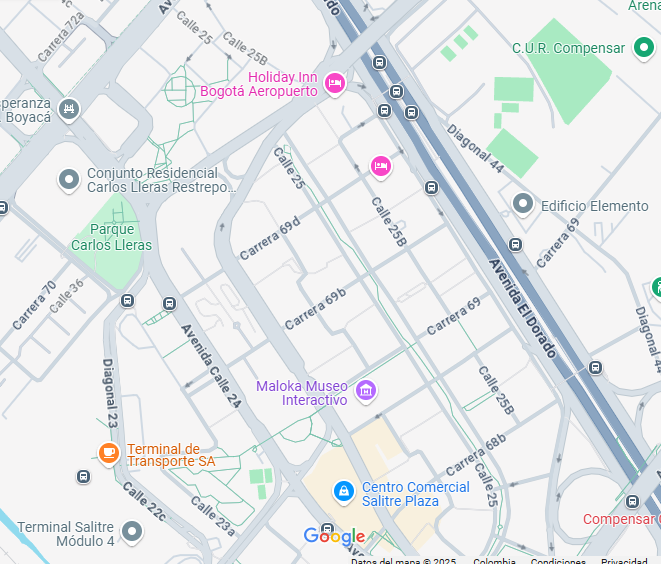
\includegraphics[width=0.37\textwidth]{temp_maps/Centro XYZ.png}
\end{center}

\newpage

\textbf{\textcolor{turquesa}{\fontsize{16}{20}\selectfont Centro XYZ – Períodos de     Retorno}}

\vspace{0.3cm}
\begin{center}
\begin{table}[!h]
\centering
\begin{tabular}{lll}
\toprule
\multicolumn{1}{>{\centering\arraybackslash}m{0.3\textwidth}}{\cellcolor{azuloscuro}{\color{white}\textbf{1-100}}} & \multicolumn{1}{>{\centering\arraybackslash}m{0.3\textwidth}}{\cellcolor{azuloscuro}{\color{white}\textbf{1-200}}} & \multicolumn{1}{>{\centering\arraybackslash}m{0.3\textwidth}}{\cellcolor{azuloscuro}{\color{white}\textbf{1-500}}}\\
\includegraphics[width=0.3\textwidth]{C:/Users/windows/Documents/GitHub/Problem_Set_1/Flood Report/Flood/1. Mapas/Cliente ABC/Centro XYZ/1-100.png} & \includegraphics[width=0.3\textwidth]{C:/Users/windows/Documents/GitHub/Problem_Set_1/Flood Report/Flood/1. Mapas/Cliente ABC/Centro XYZ/1-200.png} & \includegraphics[width=0.3\textwidth]{C:/Users/windows/Documents/GitHub/Problem_Set_1/Flood Report/Flood/1. Mapas/Cliente ABC/Centro XYZ/1-500.png}\\
\bottomrule
\end{tabular}
\end{table} 

\begin{table}[!h]
\centering
\begin{tabular}{lll}
\toprule
\multicolumn{1}{>{\centering\arraybackslash}m{0.3\textwidth}}{\cellcolor{azuloscuro}{\color{white}\textbf{1-1500}}} &  & \\
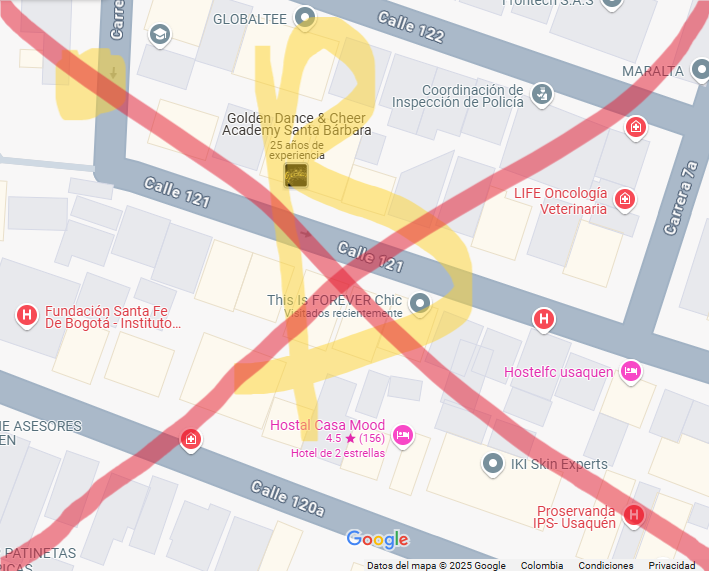
\includegraphics[width=0.3\textwidth]{C:/Users/windows/Documents/GitHub/Problem_Set_1/Flood Report/Flood/1. Mapas/Cliente ABC/Centro XYZ/1-1500.png} &  & \\
\bottomrule
\end{tabular}
\end{table} 

\end{center}
\vspace{0.5cm}
\clearpage

\noindent
\includegraphics[width=3cm]{Logo.png}

\vspace{1cm}

\noindent\textbf{\textcolor{azuloscuro}{\fontsize{28}{32}\selectfont Descarga de Responsabilidad}}

\fontsize{11}{13}\selectfont Este documento y cualquier recomendación,
análisis, o recomendación hecha por Marsh (colectivamente el ``Análisis
de Marsh'') está dirigida únicamente a esta entidad identificada como el
destinatario (usted). Este documento contiene información confidencial
propiedad de Marsh y no podrá ser compartida con tercero alguno,
incluyendo otros productores de seguros sin el consentimiento previo y
por escrito de Marsh. Cualquier declaración relacionada con asuntos
actuariales, fiscales, contables, o legales está basada únicamente en
nuestra experiencia como corredores de seguros y consultores de riesgos,
y no deberá interpretarse como asesoría, por tanto, deberá consultar a
su propio asesor profesional. Cualquier modelo, análisis, o proyección
estará sujeta a sus debidas reservas y el análisis de Marsh podría
resultar materialmente afectado si cualquier condición, suposición,
información o factor resultara inexacto o incompleto o deba modificarse.

\textbf{Datos Copyright © JBA Risk Management Limited 2024. Todos los derechos reservados.}

\fontsize{11}{13}\selectfont Los datos son el resultado de la
modelización de peligros naturales que son inciertos. No se hacen
garantías sobre la integridad, corrección o actualidad de la
información. JBA no puede predecir el futuro, y todos los datos sobre
cambio climático deben ser utilizados con precaución y basados en una
comprensión sólida de las limitaciones e incertidumbres de dichos datos.

\fontsize{11}{13}\selectfont Los datos y servicios climáticos de JBA se
basan en datos de organizaciones de terceros (modelización climática)
que JBA considera científicamente creíbles y en las propias metodologías
de desarrollo robustas de JBA. Al mismo tiempo, estos modelos tienen
deficiencias y limitaciones conocidas en su representación de los
sistemas físicos relevantes y, dado que no hay observaciones del futuro,
presentan profundas incertidumbres respecto a su capacidad para simular
climas bajo posibles condiciones futuras. Al igual que los datos
disponibles de los modelos climáticos de terceros, los datos de JBA son
solo una ilustración de uno de los muchos cambios posibles que podrían
ocurrir basados en uno o más escenarios climáticos idealizados. En
consecuencia, JBA no puede ni representa, garantiza o asegura la
precisión de la salida, sus indicaciones y estimaciones.

\fontsize{11}{13}\selectfont No debe:

\begin{itemize}
  \item Utilizar los datos de JBA o los resultados de la evaluación con fines comerciales.
  \item Proporcionar los datos de JBA o los resultados de la evaluación, en su totalidad o en parte, a ningún tercero, excepto como parte de actividades de corretaje de seguros o para fines de informes externos, documentación regulatoria o según lo exija la ley.
\end{itemize}

\end{document}
